% Options for packages loaded elsewhere
\PassOptionsToPackage{unicode}{hyperref}
\PassOptionsToPackage{hyphens}{url}
\PassOptionsToPackage{dvipsnames,svgnames,x11names}{xcolor}
%
\documentclass[
  letterpaper,
  DIV=11,
  numbers=noendperiod]{scrartcl}

\usepackage{amsmath,amssymb}
\usepackage{iftex}
\ifPDFTeX
  \usepackage[T1]{fontenc}
  \usepackage[utf8]{inputenc}
  \usepackage{textcomp} % provide euro and other symbols
\else % if luatex or xetex
  \usepackage{unicode-math}
  \defaultfontfeatures{Scale=MatchLowercase}
  \defaultfontfeatures[\rmfamily]{Ligatures=TeX,Scale=1}
\fi
\usepackage{lmodern}
\ifPDFTeX\else  
    % xetex/luatex font selection
\fi
% Use upquote if available, for straight quotes in verbatim environments
\IfFileExists{upquote.sty}{\usepackage{upquote}}{}
\IfFileExists{microtype.sty}{% use microtype if available
  \usepackage[]{microtype}
  \UseMicrotypeSet[protrusion]{basicmath} % disable protrusion for tt fonts
}{}
\makeatletter
\@ifundefined{KOMAClassName}{% if non-KOMA class
  \IfFileExists{parskip.sty}{%
    \usepackage{parskip}
  }{% else
    \setlength{\parindent}{0pt}
    \setlength{\parskip}{6pt plus 2pt minus 1pt}}
}{% if KOMA class
  \KOMAoptions{parskip=half}}
\makeatother
\usepackage{xcolor}
\setlength{\emergencystretch}{3em} % prevent overfull lines
\setcounter{secnumdepth}{-\maxdimen} % remove section numbering
% Make \paragraph and \subparagraph free-standing
\ifx\paragraph\undefined\else
  \let\oldparagraph\paragraph
  \renewcommand{\paragraph}[1]{\oldparagraph{#1}\mbox{}}
\fi
\ifx\subparagraph\undefined\else
  \let\oldsubparagraph\subparagraph
  \renewcommand{\subparagraph}[1]{\oldsubparagraph{#1}\mbox{}}
\fi


\providecommand{\tightlist}{%
  \setlength{\itemsep}{0pt}\setlength{\parskip}{0pt}}\usepackage{longtable,booktabs,array}
\usepackage{calc} % for calculating minipage widths
% Correct order of tables after \paragraph or \subparagraph
\usepackage{etoolbox}
\makeatletter
\patchcmd\longtable{\par}{\if@noskipsec\mbox{}\fi\par}{}{}
\makeatother
% Allow footnotes in longtable head/foot
\IfFileExists{footnotehyper.sty}{\usepackage{footnotehyper}}{\usepackage{footnote}}
\makesavenoteenv{longtable}
\usepackage{graphicx}
\makeatletter
\def\maxwidth{\ifdim\Gin@nat@width>\linewidth\linewidth\else\Gin@nat@width\fi}
\def\maxheight{\ifdim\Gin@nat@height>\textheight\textheight\else\Gin@nat@height\fi}
\makeatother
% Scale images if necessary, so that they will not overflow the page
% margins by default, and it is still possible to overwrite the defaults
% using explicit options in \includegraphics[width, height, ...]{}
\setkeys{Gin}{width=\maxwidth,height=\maxheight,keepaspectratio}
% Set default figure placement to htbp
\makeatletter
\def\fps@figure{htbp}
\makeatother

\KOMAoption{captions}{tableheading}
\makeatletter
\makeatother
\makeatletter
\makeatother
\makeatletter
\@ifpackageloaded{caption}{}{\usepackage{caption}}
\AtBeginDocument{%
\ifdefined\contentsname
  \renewcommand*\contentsname{Indice}
\else
  \newcommand\contentsname{Indice}
\fi
\ifdefined\listfigurename
  \renewcommand*\listfigurename{Elenco delle Figure}
\else
  \newcommand\listfigurename{Elenco delle Figure}
\fi
\ifdefined\listtablename
  \renewcommand*\listtablename{Elenco delle Tabelle}
\else
  \newcommand\listtablename{Elenco delle Tabelle}
\fi
\ifdefined\figurename
  \renewcommand*\figurename{Figura}
\else
  \newcommand\figurename{Figura}
\fi
\ifdefined\tablename
  \renewcommand*\tablename{Tabella}
\else
  \newcommand\tablename{Tabella}
\fi
}
\@ifpackageloaded{float}{}{\usepackage{float}}
\floatstyle{ruled}
\@ifundefined{c@chapter}{\newfloat{codelisting}{h}{lop}}{\newfloat{codelisting}{h}{lop}[chapter]}
\floatname{codelisting}{Lista}
\newcommand*\listoflistings{\listof{codelisting}{Elenco degli Elenchi}}
\makeatother
\makeatletter
\@ifpackageloaded{caption}{}{\usepackage{caption}}
\@ifpackageloaded{subcaption}{}{\usepackage{subcaption}}
\makeatother
\makeatletter
\@ifpackageloaded{tcolorbox}{}{\usepackage[skins,breakable]{tcolorbox}}
\makeatother
\makeatletter
\@ifundefined{shadecolor}{\definecolor{shadecolor}{rgb}{.97, .97, .97}}
\makeatother
\makeatletter
\makeatother
\makeatletter
\makeatother
\ifLuaTeX
\usepackage[bidi=basic]{babel}
\else
\usepackage[bidi=default]{babel}
\fi
\babelprovide[main,import]{italian}
% get rid of language-specific shorthands (see #6817):
\let\LanguageShortHands\languageshorthands
\def\languageshorthands#1{}
\ifLuaTeX
  \usepackage{selnolig}  % disable illegal ligatures
\fi
\IfFileExists{bookmark.sty}{\usepackage{bookmark}}{\usepackage{hyperref}}
\IfFileExists{xurl.sty}{\usepackage{xurl}}{} % add URL line breaks if available
\urlstyle{same} % disable monospaced font for URLs
\hypersetup{
  pdftitle={Le molte guerre combattute sul corpo di Imane Khelif},
  pdfauthor={Claudio Comandini},
  pdflang={it},
  colorlinks=true,
  linkcolor={blue},
  filecolor={Maroon},
  citecolor={Blue},
  urlcolor={Blue},
  pdfcreator={LaTeX via pandoc}}

\title{Le molte guerre combattute sul corpo di Imane Khelif}
\author{Claudio Comandini}
\date{10 agosto 2024}

\begin{document}
\maketitle
\ifdefined\Shaded\renewenvironment{Shaded}{\begin{tcolorbox}[sharp corners, enhanced, borderline west={3pt}{0pt}{shadecolor}, interior hidden, frame hidden, breakable, boxrule=0pt]}{\end{tcolorbox}}\fi

\begin{figure}

{\centering 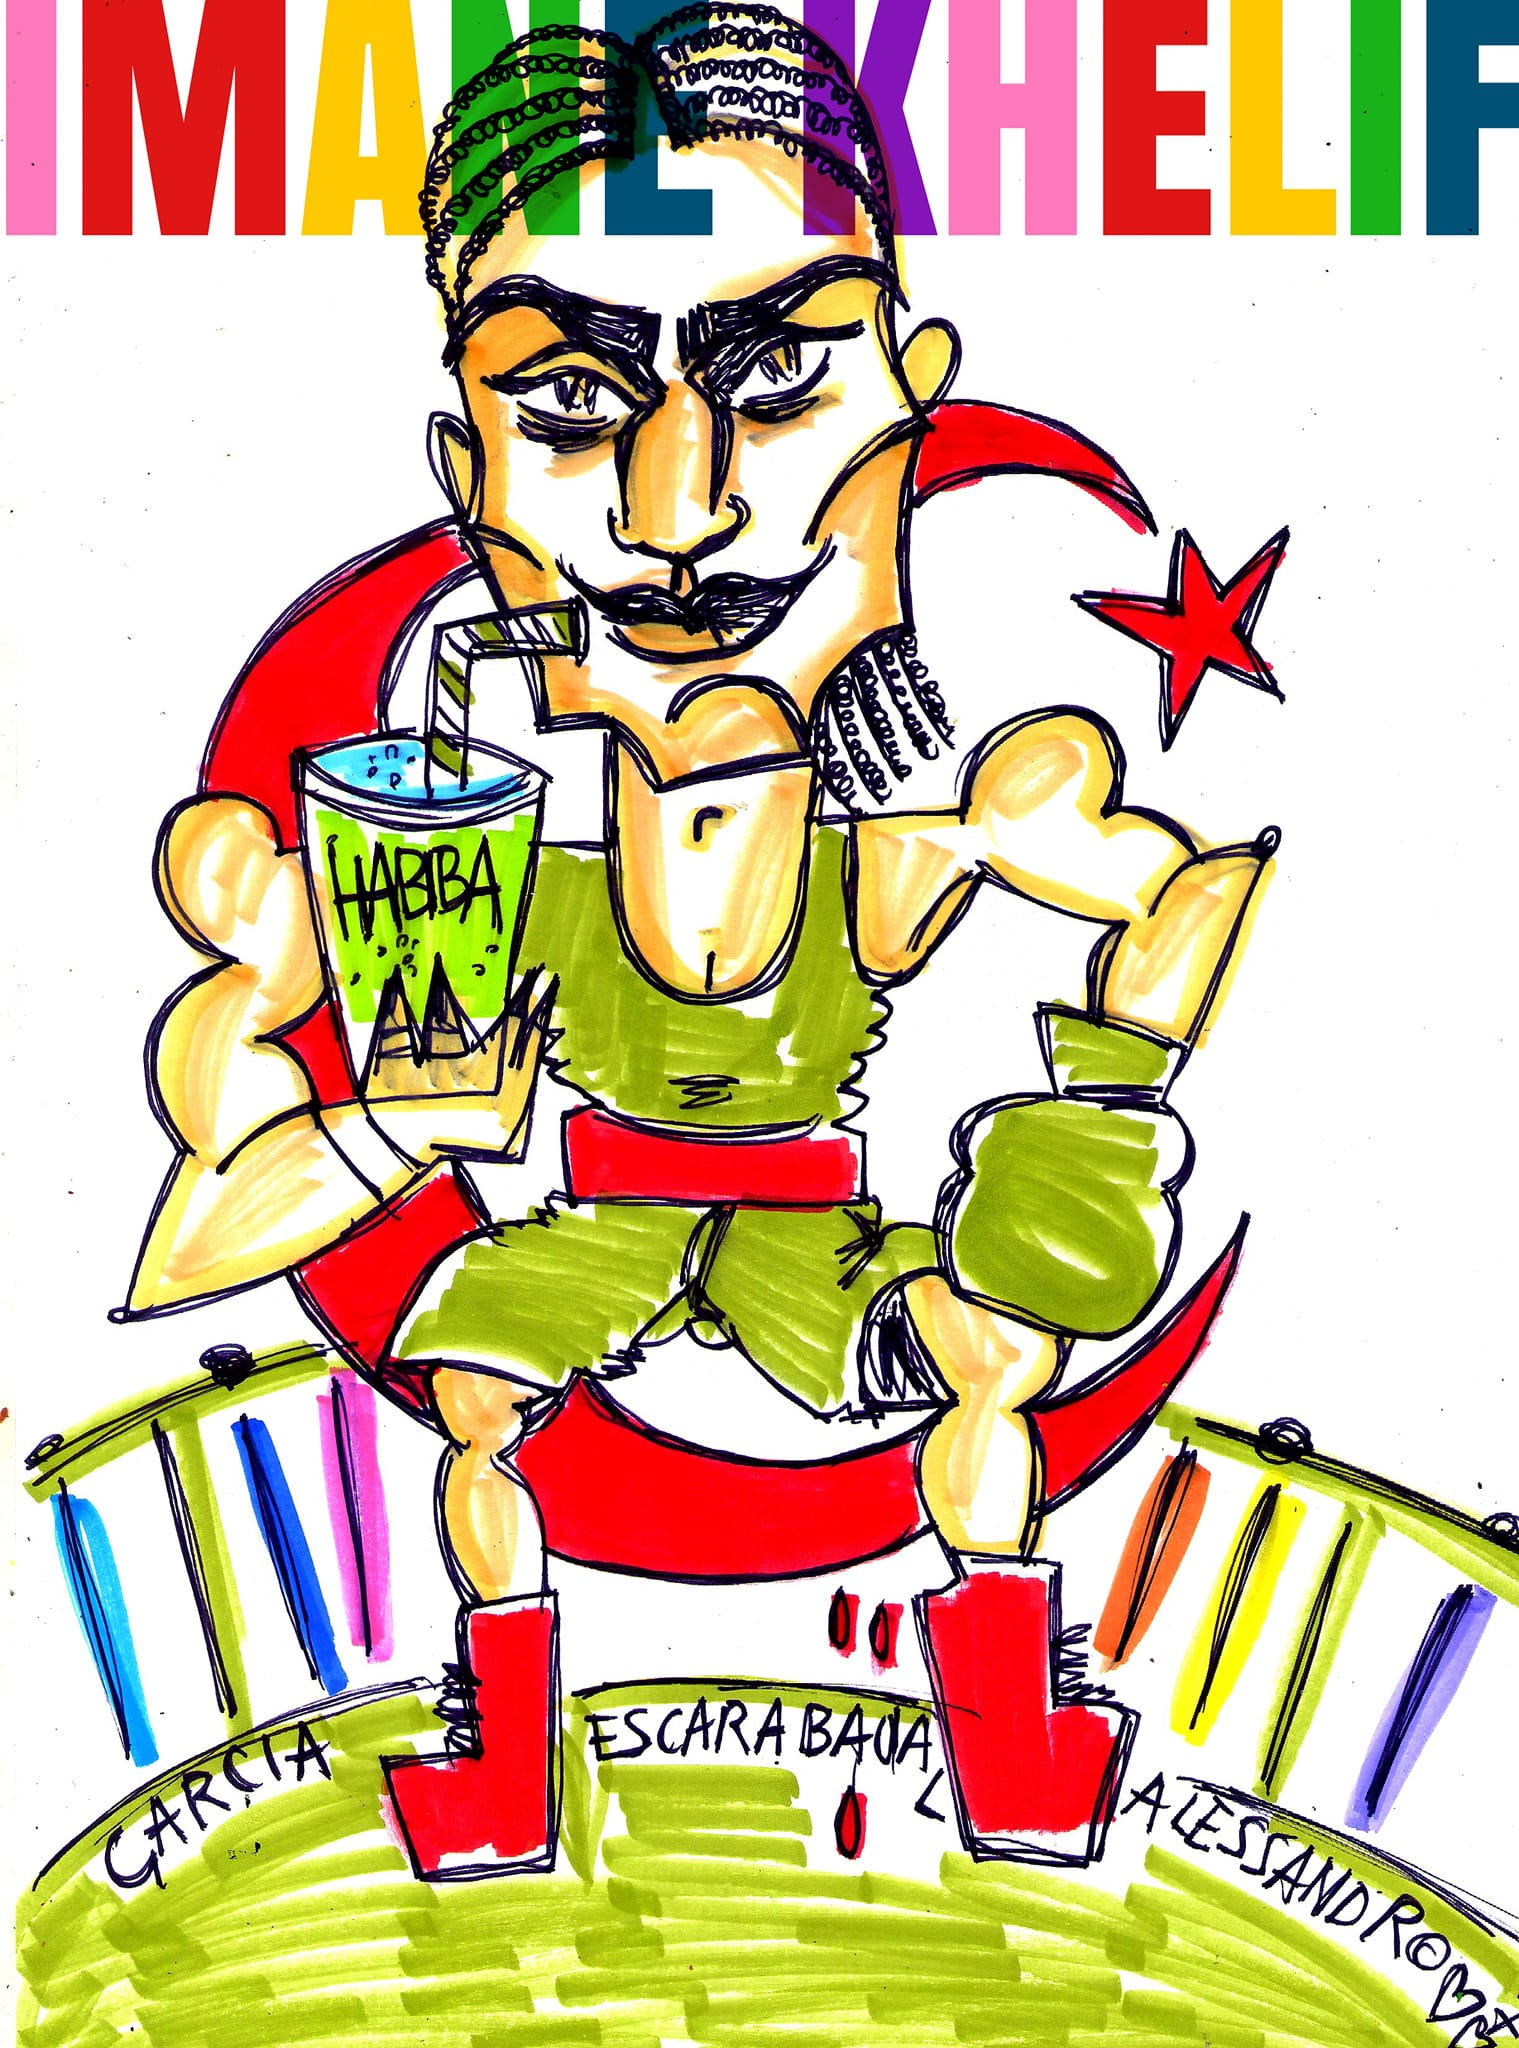
\includegraphics{images/Imane_Khelif.jpg}

}

\end{figure}

\emph{Il caos come sistema di potere. Statuti provvisori sulle donne e
la boxe. I progressisti, i regressisti e le interessate polemiche della
pubblica ottusità. Sport e parametri. Sessi e generi nella prospettiva
islamica. Conflitti di potere sul corpo di una donna. L'Italia al
tappeto.}

La deliberata e sistematica produzione di caos sembra oggi essere la
prassi più diffusa, tanto nelle guerre quanto nella comunicazione, ormai
avvezze a scambiarsi continuamente di posto. L'incertezza è
paradossalmente diventata una certezza della quale esiste misura e
contabilità, e i conti in definitiva non sono complessi laddove per
comprendere l'andazzo generale si può valutare l'interesse prevalente e
chi più ci guadagna. Tale tipo di incertezza perlopiù non provoca
interrogativi, ma piuttosto arriva a permettere a chiunque di affermare
le proprie inappellabili certezze e anzi, maggiori sono le incertezze
più impazzano le certezze, e c'è un appello generale, indipendentemente
da quanto realmente se ne possa sapere di un qualcosa, a formulare
illazioni su illazioni e merda per tutti.

Esemplare è il caso della pugile algerina Imane Khelif, categoria pesi
leggeri, partecipante alle olimpiadi 2024, trattata peggio di un
punching ball da un'opinione pubblica polarizzata senza scampo o
mediazione in \emph{progressisti} e \emph{regressisti,} ambedue distanti
dall'avere cognizione della sua effettiva condizione e parimenti
interessati a manipolarla a favore delle proprie goffe e meschine
credenze. La boxe, per quanto tradizionalmente non sia mai esattamente
stata un'occupazione per signorine, rimane comunque la \emph{noble art},
generalmente svolta da gente quantomeno svelta, anche quando riguarda
donne che picchiano altre donne. E se nella sua carriera Imane le botte
le ha date ma le ha pure prese senza riceverne troppe complicazioni, i
cazzottoni della pubblica ottusità sono ignobili e sembrano rendere
sempre più stupidi.

Ogni comprensione pone anche la questione dei criteri di giudizio su cui
si fonda e quindi dei parametri di riferimento, e certamente lo sport ne
ha di peculiari, laddove il suo principio è quello di superare i limiti.
A complicare le cose, le stesse associazioni sportive ne applicano di
diversi. Infatti, da parte loro, i protocolli CIO (Comité International
Olympique) hanno soglie di accettabilità tali da convalidare negli
atleti di ogni sesso livelli di allenamento che portano inevitabilmente
ad alta produzione di testosterone, e inoltre un doping da overdose già
è stato prassi. Invece, per quanto riguarda le analisi dell'IBA
(International Boxing Association), che avrebbero riscontrato cromosomi
sessuali XY nella pugile in occasione delle competizioni in Turchia del
2022 e in India del 2023, metodi e laboratori non sono stati nemmeno
nominati, a quanto sembra sono stati richiesti dopo la sconfitta di una
pugile russa, e contro la loro stessa autorità hanno prodotto effetti di
esclusione soltanto parziali. Inoltre, alcuni referti degli ospedali di
Parigi e Algeri dello stesso anno riferirebbero che la pugile sarebbe
affetta di un disturbo chiamato insufficienza della 5-alfa, per essere
quindi fornita, oltre che di cromosomi XY, di testicoli interni, e dove
se l'utero sarebbe assente avremmo pure un micropene. Risulta però anche
che tali rapporti sembrano ignorati dagli stessi medici ai quali sono
attributi. Insomma, a rendere questo caso di \emph{infodemia}
particolarmente complicato è dove alla campagna di diffamazione si
aggiunge il lavoro degli aggregatori di notizie. E il problema più
grande è che è questa immondizia ad attirare di più i consumatori di
notizie.

Quanto va quindi considerato è che i parametri, oltre a essere
variabili, possono essere in conflitto tra loro e derivare da altri
conflitti più generali e spietati, che in questo caso sono marcatamente
di carattere culturale e geopolitico. Di fatto, è netto il contrasto che
coinvolge da una parte il CIO, che per una visione ultraliberista del
diritto non effettua, come ricorda il portavoce Mark Adams, test sul DNA
atti a rilevare il sesso dei partecipanti, e dell'altra l'IBA, peraltro
attualmente bandito dall'organizzazione delle olimpiadi per problemi di
governance e corruzione, sponsorizzata da Gazprom e controllata da Umar
Kremlev, oligarca del Tagikistan vicino a Putin.

I parametri sono utili per definire la realtà, ed è necessario
stabilirli con sempre maggiore accuratezza affinché si salvaguardi il
senso della competizione sportiva e il modo adeguato per parteciparvi,
ma certamente nessuno di tali parametri, che cambiano anche in ragione
di quanto lo sport richieda prestazioni sempre più elevate, può
sostituire una realtà che esiste di per sè, con tutte le sue infinite
variazioni. Insomma, tale questione ha messo in risalto l'esistenza
delle persone intersessuali, tra loro piuttosto diversificate. Senza
ripercorrere le attenzioni che possono aver ricevuto da studiosi quali
Foucault o la Butler, dobbiamo chiederci questo: occorre inventare per
ognuno di loro una categoria peculiare, oppure riconoscere loro il
genere nei cui confronti sviluppano la massima similiarità
riscontrabile?

Nella generale incertezza, su questo specifico caso qualche informazione
maggiormente riscontrabile di altre la abbiamo per davvero. Infatti,
nonostante sembri avere peculiarità nella produzione ormonale e sia di
aspetto mascolino, la venticinquenne, oltre oltre ad avere donna scritto
sul passaporto e ad aver sempre vissuto da donna, non esprime una
condizione transgender, non ha fatto nessuna transizione e nemmeno ne è
lontanamente interessata. Probabilmente, neanche la ritiene possibile e
altresì non ha alcun bisogno che qualcuno di una cultura che le è
estranea e che non la interessa minimamente ne difenda qualche diritto o
roba del genere. Probabilmente, è affetta dalla femminilissima sindrome
dell'ovaio policistico, che colpisce tra l'8 e il 13 per cento delle
donne determinando forme di iperandroginia.

Ad ogni modo, il dato decisivo, che sembra essere sfuggito a tutti, è
che, per quanto sia stata fatta oggetto a livello personale da una
psicosi mediatica da pesi massimi, la pugile si sottrae dai contenuti
che la hanno investita e dalla loro stessa terminologia in qualità di
donna musulmana ed esponente rilevante di un Paese musulmano. Paese che
con la Francia che ospita le competizioni ha un rapporto problematico,
del quale è segno anche il fatto che la donna non parla francese. E
l'Algeria, che deve consolidare il proprio ruolo regionale e sedare i
contrasti interni, ha preso senza riserve le parti della sua atleta che
è già ambasciatrice UNICEF. Il supporto offerto a questo donna così
chiacchierata è stato quindi formulato piena osservanza della
\emph{sharia} e delle indicazioni della scuola giuridica
\emph{malikita}, particolarmente adattabile alle contingenze per il
ruolo che vi assume l'opinione individuale.

Per l'Islam i sessi sono diversi, distinti e complementari, la
sessualità è creazione perpetuata e funzione sacra atta a permetterci di
conoscerci a vicenda (\emph{Corano} 4:1; 49:13). Secondo tale
prospettiva, laddove sesso e genere indicano rispettivamente
l'appartenenza biologica e la tipizzazione culturale, la mancata
complementarietà e la mancata generazione vanno a determinare, piuttosto
che fluidità, isolamento e chiusura. Se concetti tipo quelli di
orientamento e la stessa omosessualità non sono neanche pensabili, le
questioni di genere possono venir considerate in termini non remoti a
pensatori occidentali quali Otto Weininger, per cui la polarità maschile
e femminile ammette gradi intermedi e mantiene un ordine archetipico, e
Ivan Illich, secondo il quale il genere completa il sesso per tendere a
rapporti di complementarietà.

Nell'impazzare delle informazioni e degli interessi che le sono
collegati, la realtà dei fatti continua a sfuggire anche dopo che la
pugile algerina, dopo aver sconfitto in successione l'italiana Angela
Carini (ritiratasi), l'ungherese Luca Hamori (che l'aveva insultata via
social), la thailandese Janjaem Suwannapheng (che l'ha abbracciata
insieme a tutto il suo staff) e quindi la cinese Yang Liu (rimasta in
balia di un 5-0 netto), ha vinto l'oro in queste olimpiadi 2024, giocate
sulla contrapposzione ideologica più becera. Resta incerto anche il
perché la sua collega taiwanese Lin-Yu-Ting, a detta dell'IBA a sua
volta caso controverso per quanto nemmeno lei mai ufficialmente
appellata quale trans, se ne sia parlato molto meno e con toni
decisamente meno violenti, ma è probabile che ciò dipenda dai Paesi
coinvolti nelle competizioni sportive e dal loro livello di permeabilità
alle polemiche e alle strumentalizzazioni. Questa realtà ha intrecciato
conflitti di identità, cultura e civiltà sul corpo di Imane che, nel suo
autodefinirsi «\emph{donna forte e con poteri speciali}» ha sempre
continuato a riconoscersi, senza troppe complicazioni, quale donna per
quindi dedicare la sua stessa battaglia alle donne tutte, attraversando
accuse e umiliazioni che hanno dato alla sua vittoria «\emph{un sapore
speciale}».

Tutto è molto complesso e incerto e il caos non ha risparmiato nessuno,
indipendentemente da quanto ognuno della vicenda complessiva ne abbia
compreso. Un branco ha inappellabilmente deciso che Imane sia un uomo, e
lo ha fatto soltanto per odiare, e continuerà a farlo pure se si gli
presentasse davanti nuda con le analisi del DNA stampate
sull'\emph{hijab}. Un altro branco non trova meglio da fare che accusare
la Russia di questa epidemia di stronzate, perché la Russia è cattiva e
loro sono buoni e vogliono tanto bene ai diversi, pure se nemmeno
capiscono di cosa stanno parlando. Progressisti e regressisti sono
schieramenti incomunicanti eppure interdipendenti di un \emph{logos}
sepolto, ombre che proiettano ombre senza vedere altro che la distorta
proiezione di se stessi. Ad ogni modo, se questa epidemia ha un
epicentro, per quanto abbia colpito eminenze quali Musk e la Rowling,
questo è l'Italia, e se conosce un ``\emph{paziente zero}'' questi è
Salvini, almeno ufficialmente il primo a cadere su X in un equivoco che
sembrerebbe comunque orchestrato altrove proprio per creare quel caos
con cui oggi si pretende di controllare il mondo. E certamente anche ciò
è piuttosto incerto. Indipendentemente da ogni dato possa venir prodotto
e da ogni ragionamento compiuto possa venir articolato, tutte le
incertezze restano sempre e comunque in piedi, sempre pronte ad essere
smentite, per lasciare così ognuno in preda alla propria immaginazione
ad alimentare, spesso suo malgrado, lo stesso caos che è costretto a
subire.

Ad ogni modo, per quanto la situazione resti complessa, non ci vuole
molto a capirne i significati più stringenti: l'equivoco chiamato
occidente è ormai andato alla deriva insieme a tutte le sue tare
pregresse e autoimmuni, ed è ormai palesemente incapace di distinguere,
li guardi da destra o da sinistra, persino il cazzo dalla fica. Da parte
sua, la rozza, pretenziosa e piagnucolosa italietta ha mostrato di sé
davvero un brutto spettacolo su ogni ring e su ogni schermo, e non serve
dilungarsi troppo ed entrare in dettagli; quanto resta è godersi il suo
dissolversi, senza farsi coinvolgere più di tanto dai suoi equivoci. E
della certezza della nostra incertezza rispetto al nostro Paese possiamo
addirittura andarne fieri tutti, uomini e donne di ogni tipo, senza
nemmeno più tanto bisogno di picchiarci. E magari verrà il tempo in cui
anche per qualcuno di noi dignità e onore verranno prima di tutto.

\emph{Illustrazione: caricatura di Imane Khelif tratta dal suo profilo
Facebook.}



\end{document}
